\section{引言}  %引言


\begin{frame}
	\frametitle{研究背景和意义}
	\begin{columns}[T] % align columns
		\begin{column}<0->{.40\textwidth}
			\begin{figure}[thpb]
				\centering
				\resizebox{1\linewidth}{!}{
					% MOT16-03
					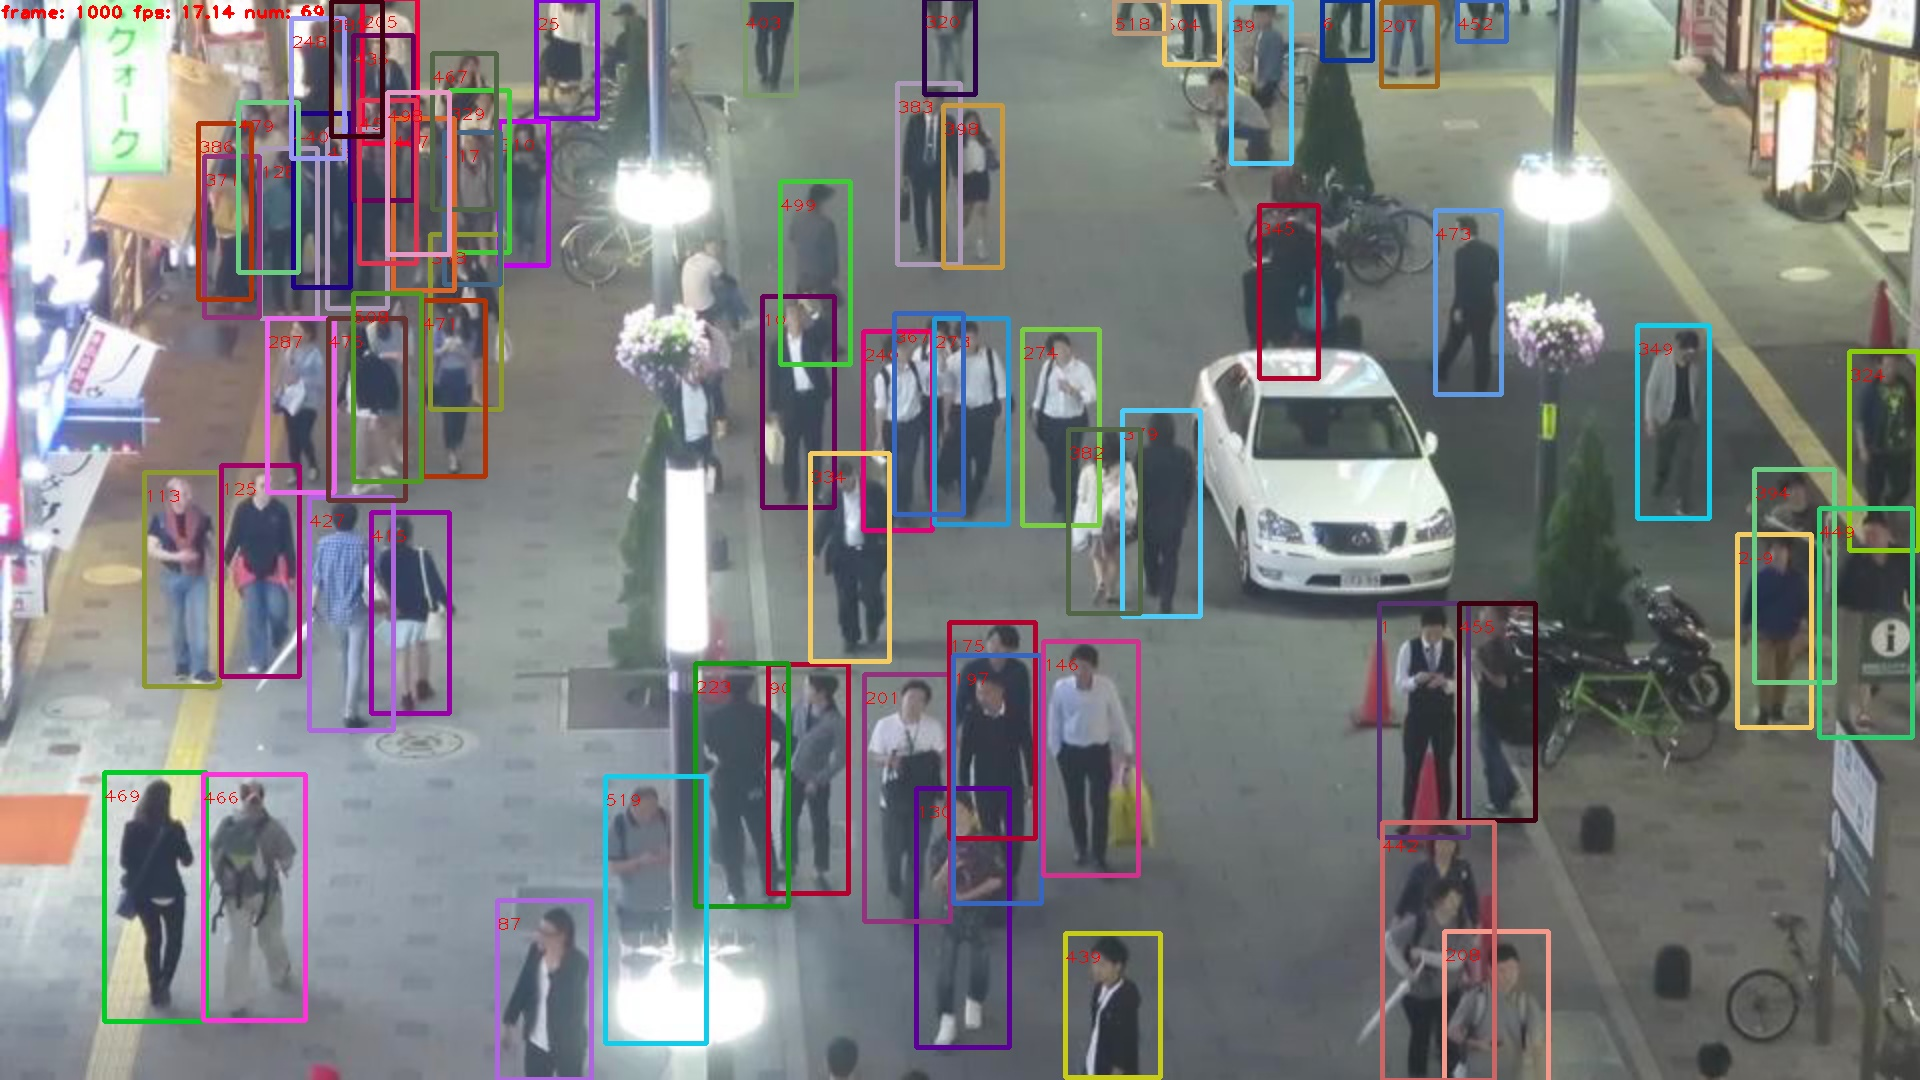
\includegraphics{figures/MOT-16-03_01000.jpg}
				}
				%\includegraphics[scale=1.0]{figurefile}
				\caption{多目标跟踪示例}
				\label{fig:campus}
			\end{figure}
		\end{column}
		\hfill%
		\begin{column}<0->{.65\textwidth}
			\begin{itemize}
				\item<1-> 复杂场景下的多目标跟踪是计算机视觉领域中基础且重要的研究方向
				\begin{itemize}
					\item<1-> 也是全球大学、研究所和公司所亟待解决的核心问题
				\end{itemize}
				% 数字表示出现的顺序
				\item<1-> 主要的应用领域
				\begin{itemize}
					\item<1-> 智能视频监控
					\item<1-> 智能驾驶
					\item<1-> 智能机器人
					\item<1-> 体育视频分析
				\end{itemize}
			\end{itemize}
		\end{column}%
	\end{columns}
\end{frame}


\begin{frame}
	\frametitle{主要问题和挑战}
	\begin{columns}[T] % align columns
		\begin{column}<0->{.40\textwidth}
			\begin{figure}[thpb]
				\centering
				\resizebox{1\linewidth}{!}{
					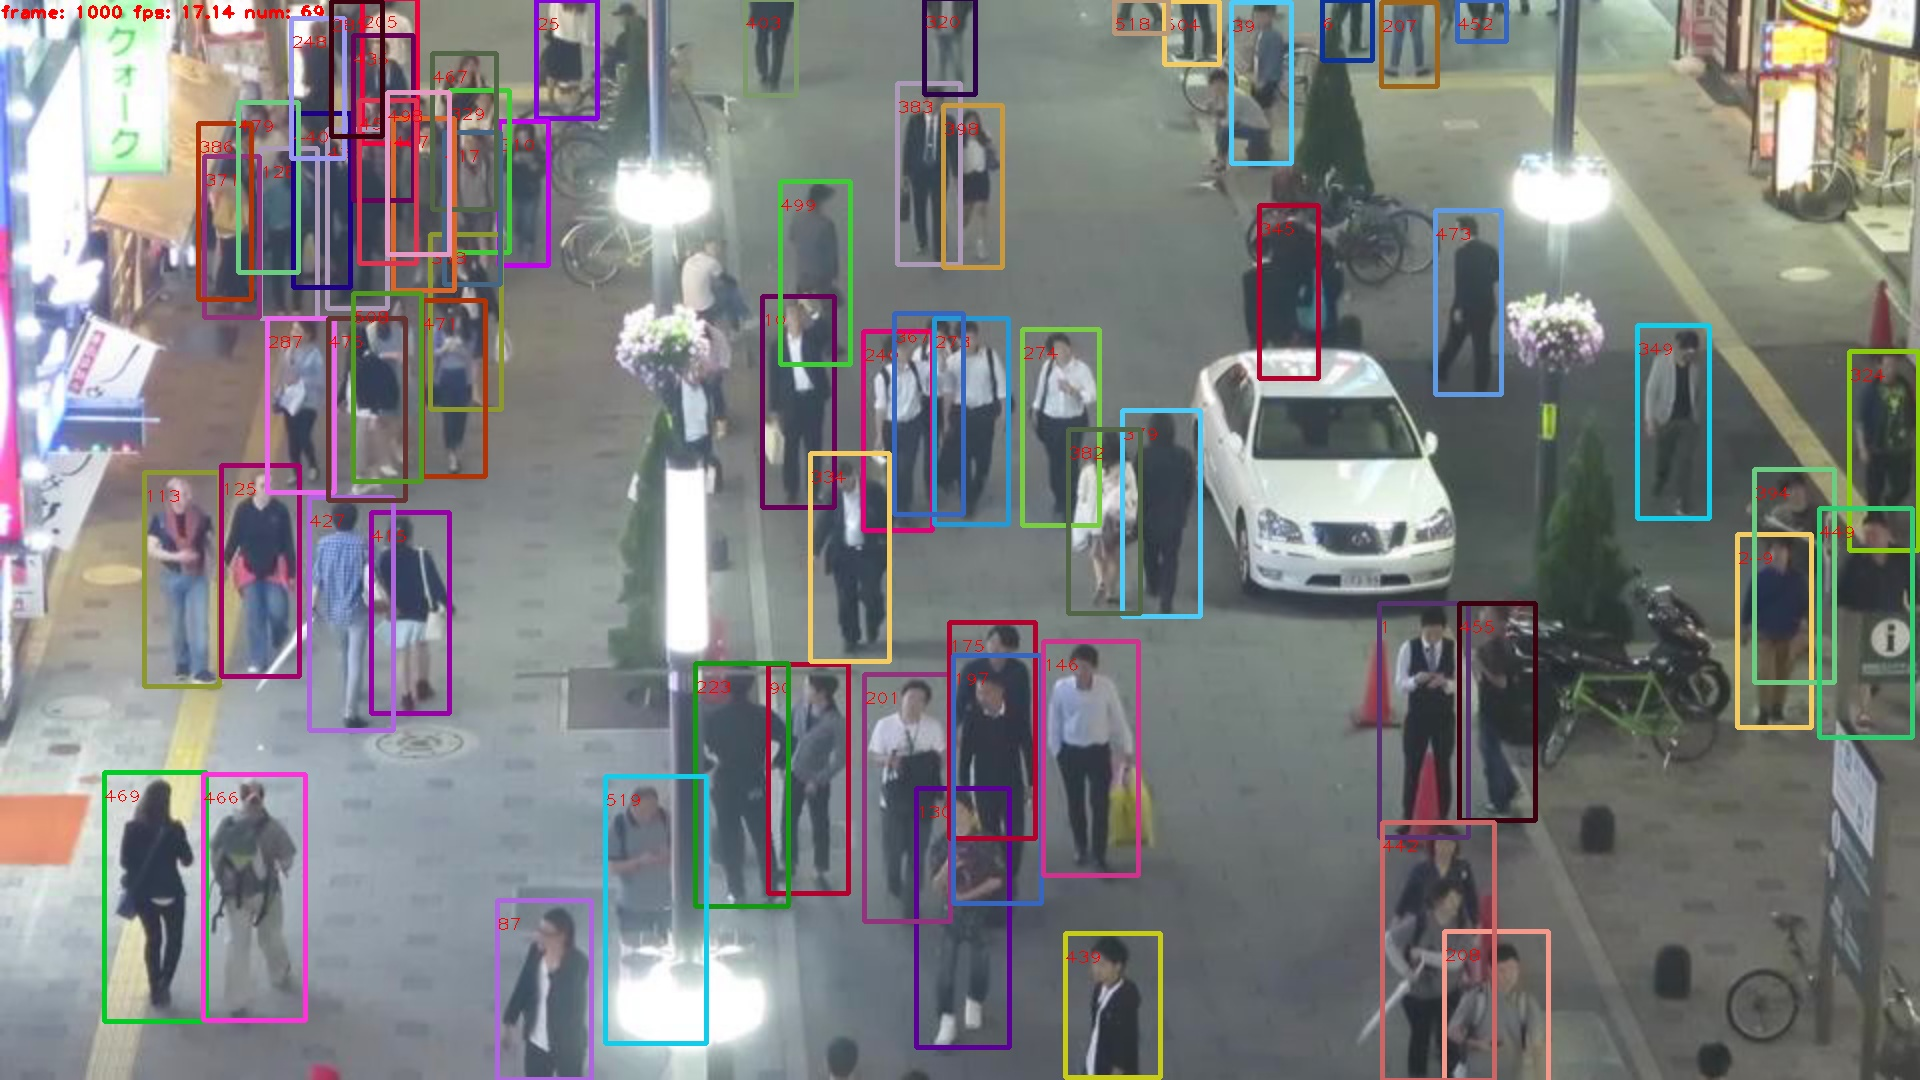
\includegraphics{figures/MOT-16-03_01000.jpg}
				}
				%\includegraphics[scale=1.0]{figurefile}
				\caption{多目标跟踪示例}
			\end{figure}
		\end{column}
		\hfill%
		\begin{column}<0->{.65\textwidth}
			\begin{itemize}
				\item<1-> 单目标跟踪算法扩展到多目标场景中的问题
				\begin{itemize}
					\item<1-> 模型复杂程度和可理解性问题
					\item<1-> 跟踪漂移问题
				\end{itemize}
				\item<1-> 基于检测的数据关联多目标跟踪算法的缺陷
				\begin{itemize}
					\item<1-> 时空特征建模的复杂性问题
					\item<1-> 检测和跟踪任务相互独立问题
				\end{itemize}
			\end{itemize}
		\end{column}%
	\end{columns}
\end{frame}


\begin{frame}
	\frametitle{本文的解决方案}
	\begin{columns}[T] % align columns
		\begin{column}<0->{.40\textwidth}
			\begin{figure}[thpb]
				\centering
				\resizebox{1\linewidth}{!}{
					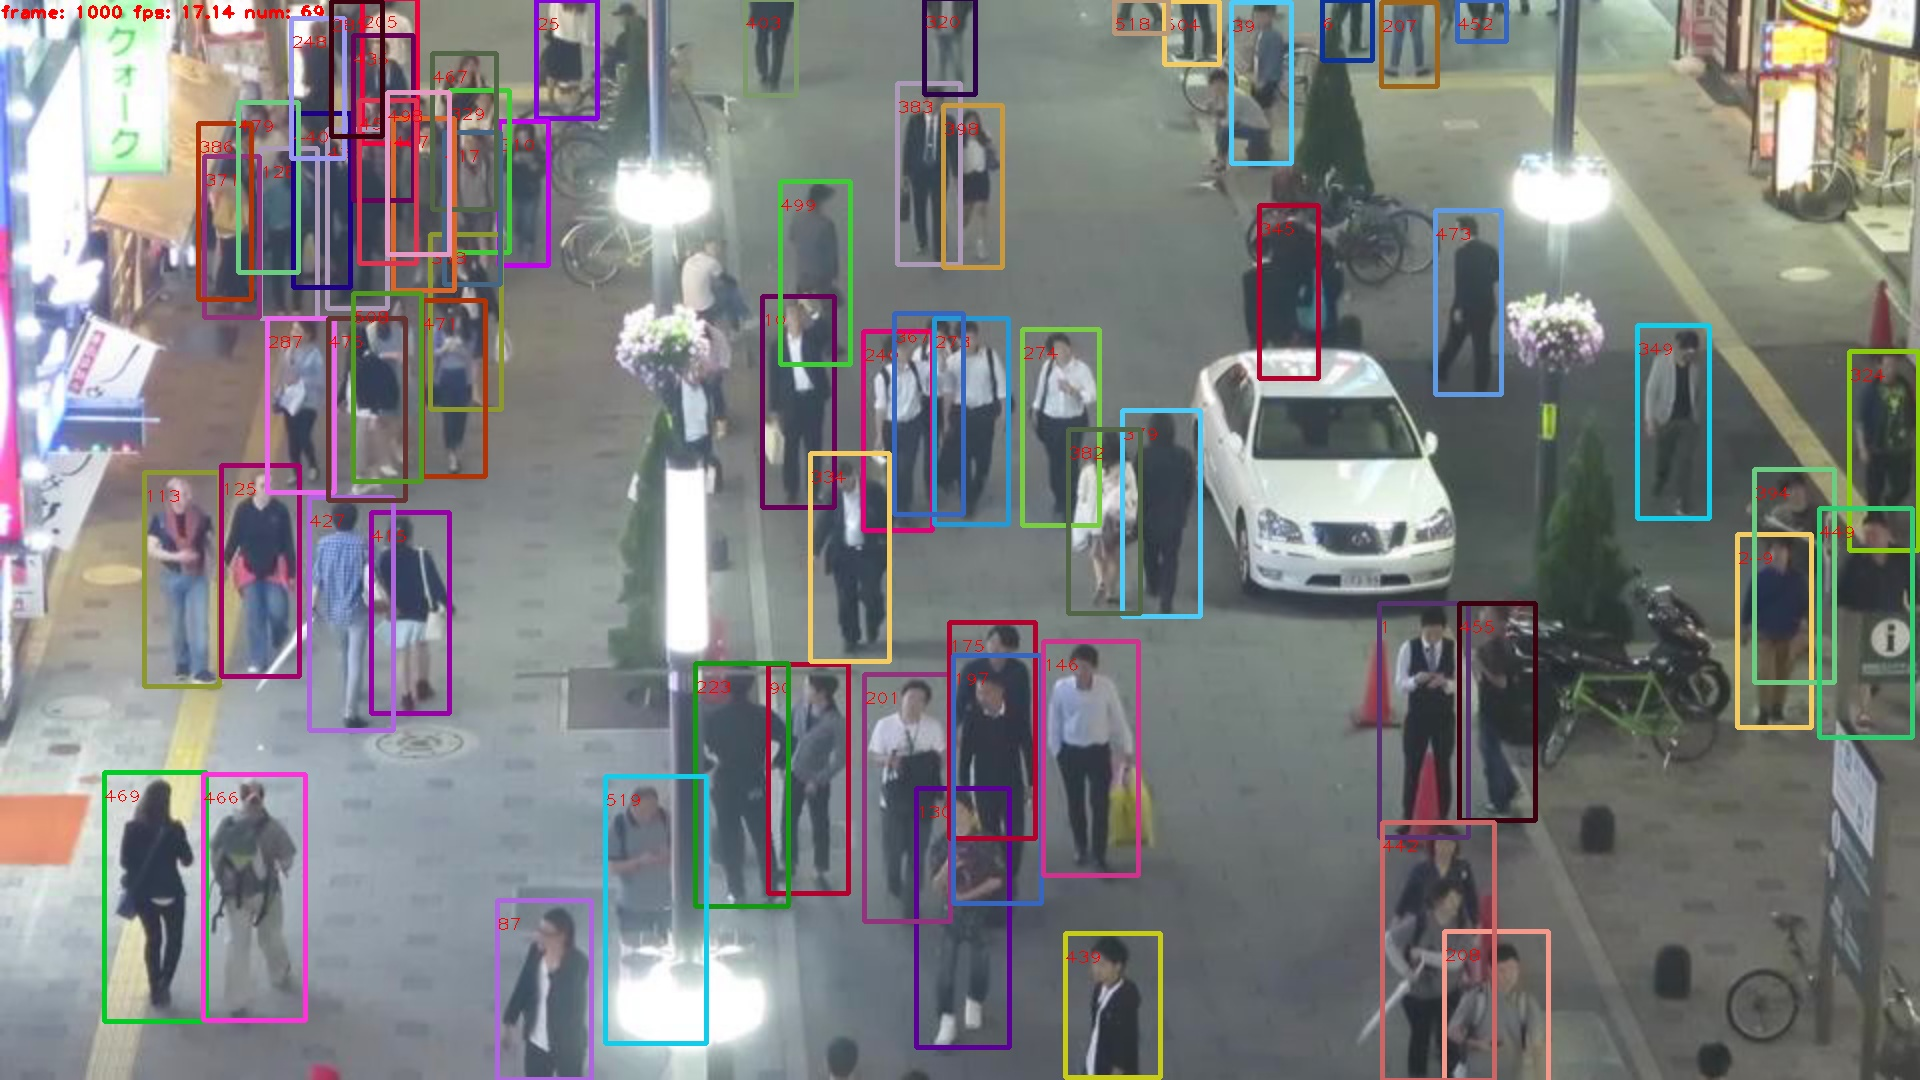
\includegraphics{figures/MOT-16-03_01000.jpg}
				}
				%\includegraphics[scale=1.0]{figurefile}
				\caption{多目标跟踪示例}
			\end{figure}
		\end{column}
		\hfill%
		\begin{column}<0->{.65\textwidth}
			\begin{itemize}
				\item<1-> 神经解剖对齐的类脑跟踪模型,来进行单目标跟踪
				% 2,3都是解决时空特征建模问题 + 漂移
				\item<1-> 跨时范围的全局注意力的模型,提升关联效果并解决漂移问题
				\item<1-> 时空互学习方法,以解决当前和历史特征不平衡的问题
				\item<1-> 端到端模型架构和训练方法,来联合检测和跟踪
				
			\end{itemize}
		\end{column}%
	\end{columns}
\end{frame}